% !TeX program = xelatex
\documentclass[a4paper,10pt]{article}

% ============================================================================
% ១. កញ្ចប់បណ្ណាល័យ និងការកំណត់ទំព័រ (Packages & Page Setup — តាមគំរូ ls_plan.tex)
% ============================================================================
\usepackage[a4paper, left=0.95cm, right=0.95cm, top=0.85cm, bottom=0.92cm, footskip=0.52cm]{geometry}
\usepackage{amsmath}
\usepackage{unicode-math}
\usepackage{fontspec}
\usepackage{longtable, array, multirow, colortbl}
\usepackage[table]{xcolor}
\usepackage{enumitem}
\usepackage{pifont}
\usepackage{fancyhdr}
\usepackage{tikz}
\usetikzlibrary{calc, arrows.meta, decorations.pathreplacing, patterns, positioning, babel}

\makeatletter
\let\@expl@@@mark@update@singlecol@structures@@\relax
\makeatother

% --- ប្រព័ន្ធស្វែងរកទីតាំងពុម្ពអក្សរស្វ័យប្រវត្តិ (Windows Local + Cloud Repo fonts/) ---
\providecommand{\NGSFindFonts}{%
  \IfFileExists{C:/Windows/Fonts/cambria.ttc}{%
    \def\NGSSysPath{C:/Windows/Fonts/}%
    \def\NGSUserPath{C:/Users/KIT/AppData/Local/Microsoft/Windows/Fonts/}%
  }{%
    \IfFileExists{./fonts/KhmerOSsiemreap.ttf}{\def\NGSSysPath{./fonts/}\def\NGSUserPath{./fonts/}}{%
    \IfFileExists{../fonts/KhmerOSsiemreap.ttf}{\def\NGSSysPath{../fonts/}\def\NGSUserPath{../fonts/}}{%
    \IfFileExists{../../fonts/KhmerOSsiemreap.ttf}{\def\NGSSysPath{../../fonts/}\def\NGSUserPath{../../fonts/}}{%
    \IfFileExists{../../../fonts/KhmerOSsiemreap.ttf}{\def\NGSSysPath{../../../fonts/}\def\NGSUserPath{../../../fonts/}}{%
    \IfFileExists{../../../../fonts/KhmerOSsiemreap.ttf}{\def\NGSSysPath{../../../../fonts/}\def\NGSUserPath{../../../../fonts/}}{%
    \IfFileExists{../../../../../fonts/KhmerOSsiemreap.ttf}{\def\NGSSysPath{../../../../../fonts/}\def\NGSUserPath{../../../../../fonts/}}{%
    \IfFileExists{../../../../../../fonts/KhmerOSsiemreap.ttf}{\def\NGSSysPath{../../../../../../fonts/}\def\NGSUserPath{../../../../../../fonts/}}{%
      \def\NGSSysPath{../../../../../../../fonts/}\def\NGSUserPath{../../../../../../../fonts/}%
    }}}}}}}%
  }%
}
\NGSFindFonts

% ============================================================================
% ២. កំណត់ពុម្ពអក្សរ (Fonts — តាមគំរូ ls_plan.tex)
% ============================================================================
\setmathfont[Path={\NGSSysPath}, FontIndex=1, Scale=1.02]{cambria.ttc}
\defaultfontfeatures{Ligatures=TeX}

\setmainfont[
  Path={\NGSUserPath},
  Extension=.ttf,
  Script=Khmer,
  BoldFont={KhmerOSsiemreap},
  BoldFeatures={FakeBold=1.8},
  ItalicFont={KhmerOSsiemreap},
  ItalicFeatures={FakeSlant=0.25},
  BoldItalicFont={KhmerOSsiemreap},
  BoldItalicFeatures={FakeBold=1.8, FakeSlant=0.25}
]{KhmerOSsiemreap}

\newfontfamily\muol[Path={\NGSUserPath}, Extension=.ttf, Script=Khmer]{KhmerOSmuollight}
\newfontfamily\Tacteing[Path={\NGSUserPath}, Extension=.TTF]{TACTENG}
\newfontfamily\TimesEn[Path={\NGSSysPath}, Extension=.ttf, BoldFont={timesbd}, ItalicFont={timesi}, BoldItalicFont={timesbi}]{times}
\newfontfamily\CalibriFont[Path={\NGSSysPath}, Extension=.ttf]{calibri}
\newfontfamily\CourierCirc[Path={\NGSSysPath}, Extension=.ttf]{cour}

\XeTeXlinebreaklocale "km"
\XeTeXlinebreakskip = 0pt plus 1pt minus 0.1pt

% ============================================================================
% ៣. ពណ៌ និងការតុបតែង (Colors & Styles)
% ============================================================================
\definecolor{stepbg}{HTML}{D9D9D9}
\definecolor{headgray}{HTML}{E6E6E6}
\definecolor{emphred}{HTML}{C00000}

\pagestyle{fancy}
\fancyhf{}
\renewcommand{\headrulewidth}{0pt}
\fancyfoot[R]{\CalibriFont\fontsize{9pt}{11pt}\selectfont\thepage}

\setlength{\parindent}{0pt}
\setlength{\parskip}{0pt}
\setlength{\tabcolsep}{4.5pt}
\setlength{\LTpre}{2pt}
\setlength{\LTpost}{2pt}

\newcolumntype{L}[1]{>{\raggedright\arraybackslash}p{#1}}
\newcolumntype{C}[1]{>{\centering\arraybackslash}p{#1}}

% ============================================================================
% ៤. ពាក្យបញ្ជាជំនួយ (Helper Macros)
% ============================================================================
\newcommand{\en}[1]{{\TimesEn #1}}
\newcommand{\enbf}[1]{{\TimesEn\bfseries #1}}
\newcommand{\khmflourish}{{\Tacteing\fontsize{15pt}{15pt}\selectfont 3}}
\newcommand{\wcirc}{{\CourierCirc\fontsize{9.5pt}{11pt}\selectfont o}}
\newcommand{\ditem}{{\fontsize{7.5pt}{10pt}\selectfont\ding{117}}\ }
\newcommand{\fiveE}[1]{\textcolor{emphred}{\CalibriFont\bfseries #1}}
\newcommand{\redsub}[1]{\textcolor{emphred}{#1}}
\newcommand{\timenote}[1]{\textcolor{emphred}{\textit{#1}}}
\newcommand{\stepheader}[1]{\multicolumn{3}{|c|}{\cellcolor{stepbg}\muol #1} \\ \hline}
\newcommand{\cfig}[1]{{\centering\vspace{3pt}#1\vspace{3pt}\par}}
\newcommand{\cnum}[1]{\mbox{\fontsize{10.5pt}{12pt}\selectfont\ding{\numexpr181+#1\relax}}}
\newcommand{\unit}[1]{\,\text{\en{#1}}}
\newcommand{\graybox}[1]{\colorbox{headgray}{\strut #1}}

% ============================================================================
% ៥. រូបភាព TikZ ស-ខ្មៅ សម្រាប់បង្រៀនលើក្ដារខៀន និងសន្លឹកកិច្ចការ (B&W Diagrams)
% ============================================================================

% ១. E1 Engage: អន្ទាក់ធ្វើវិធីបូកមុនដកក្នុង 19 - 3 + 7 (ឧទាហរណ៍ ១ ទំ.៩)
\newcommand{\figEngageWNOneFive}{%
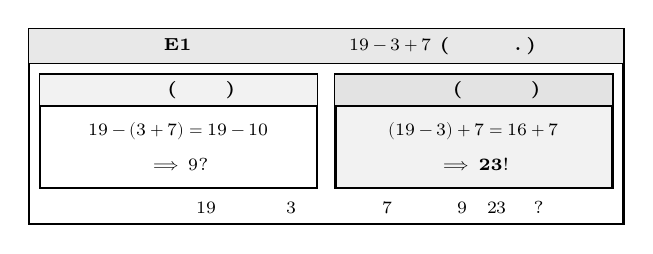
\begin{tikzpicture}[x=1cm, y=1cm, every node/.style={font=\fontsize{6.3pt}{8.3pt}\selectfont, text=black}]
  \draw[black, line width=0.9pt] (0,0) rectangle (7.55,2.48);
  \fill[gray!18] (0,2.04) rectangle (7.55,2.48);
  \draw[black, line width=0.6pt] (0,2.04) -- (7.55,2.04);
  \node at (3.775,2.26) {\textbf{បេសកកម្ម \en{E1}៖ អន្ទាក់លំដាប់ប្រមាណវិធីក្នុង $19 - 3 + 7$ (ឧទាហរណ៍ ១ ទំ.៩)}};

  % Left: Student A
  \draw[black, line width=0.8pt] (0.14,0.46) rectangle (3.66,1.90);
  \fill[gray!10] (0.14,1.50) rectangle (3.66,1.90);
  \draw[black, line width=0.5pt] (0.14,1.50) -- (3.66,1.50);
  \node at (1.90,1.70) {\textbf{សិស្ស ក (ធ្វើបូកមុន)}};
  \node at (1.90,1.18) {$19 - (3 + 7) = 19 - 10$};
  \node at (1.90,0.76) {$\implies 9$?};

  % Right: Student B
  \draw[black, line width=0.95pt, fill=gray!10] (3.89,0.46) rectangle (7.41,1.90);
  \fill[gray!22] (3.89,1.50) rectangle (7.41,1.90);
  \draw[black, line width=0.55pt] (3.89,1.50) -- (7.41,1.50);
  \node at (5.65,1.70) {\textbf{សិស្ស ខ (ពីឆ្វេងទៅស្ដាំ)}};
  \node at (5.65,1.18) {$(19 - 3) + 7 = 16 + 7$};
  \node at (5.65,0.76) {$\implies \mathbf{23}$!};

  \node at (3.775,0.21) {\textbf{សំណួរ៖} មានប្រាក់ $19$ ម៉ឺន ចាយអស់ $3$ ម៉ឺន រួចបានថែម $7$ ម៉ឺន តើសល់ $9$ ឬ $23$ ម៉ឺន?};
\end{tikzpicture}}

% ២. E2 Explore: ការគូសដង្កៀបរងតាមជំហាន (ឧទាហរណ៍ ៤ និង ៥ ទំ.៩)
\newcommand{\figStepTraceWNOneFive}{%
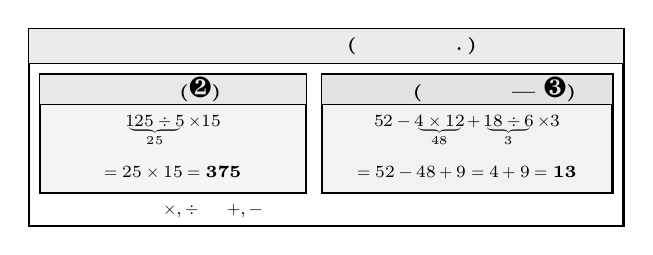
\begin{tikzpicture}[x=1cm, y=1cm, every node/.style={font=\fontsize{6.2pt}{8.2pt}\selectfont, text=black}]
  \draw[black, line width=0.9pt] (0,0) rectangle (7.55,2.50);
  \fill[gray!16] (0,2.06) rectangle (7.55,2.50);
  \draw[black, line width=0.6pt] (0,2.06) -- (7.55,2.06);
  \node at (3.775,2.28) {\textbf{ការតាមដានជំហានដោយគំនូសផ្ដុំពីក្រោម (ឧទាហរណ៍ ៤ និង ៥ ទំ.៩)}};

  % Left: Ex 4
  \draw[black, line width=0.8pt, fill=gray!8] (0.14,0.42) rectangle (3.52,1.92);
  \fill[gray!18] (0.14,1.54) rectangle (3.52,1.92);
  \draw[black, line width=0.5pt] (0.14,1.54) -- (3.52,1.54);
  \node at (1.83,1.73) {\textbf{ឧទាហរណ៍ ៤ (\cnum{2})}};
  \node at (1.83,1.22) {$\underbrace{125 \div 5}_{25} \times 15$};
  \node at (1.83,0.68) {$= 25 \times 15 = \mathbf{375}$};

  % Right: Ex 5
  \draw[black, line width=0.85pt, fill=gray!10] (3.72,0.42) rectangle (7.41,1.92);
  \fill[gray!22] (3.72,1.54) rectangle (7.41,1.92);
  \draw[black, line width=0.5pt] (3.72,1.54) -- (7.41,1.54);
  \node at (5.565,1.73) {\textbf{ឧទាហរណ៍ ៥ (ប្រមាណវិធីទាំងបួន — \cnum{3})}};
  \node at (5.565,1.22) {$52 - \underbrace{4\times 12}_{48} + \underbrace{18\div 6}_{3}\times 3$};
  \node at (5.565,0.68) {$= 52 - 48 + 9 = 4 + 9 = \mathbf{13}$};

  \node at (3.775,0.19) {ធ្វើ $\times, \div$ មុន $+, -$ ហើយក្នុងកម្រិតដូចគ្នាត្រូវគណនាពីឆ្វេងទៅស្ដាំជានិច្ច};
\end{tikzpicture}}

% ៣. E3 Explain: ឋានានុក្រម ៤ កម្រិតនៃលំដាប់ប្រមាណវិធី (ទំ.៩-១០)
\newcommand{\figHierarchyWNOneFive}{%
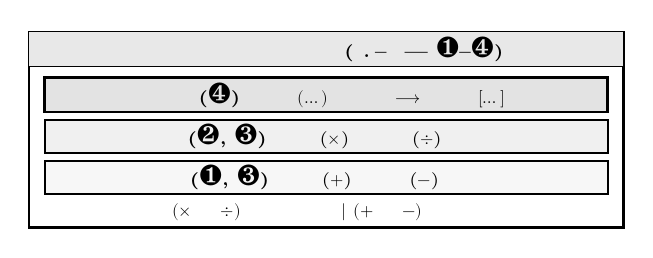
\begin{tikzpicture}[x=1cm, y=1cm, every node/.style={font=\fontsize{6.2pt}{8.1pt}\selectfont, text=black}]
  \draw[black, line width=0.9pt] (0,0) rectangle (7.55,2.48);
  \fill[gray!18] (0,2.04) rectangle (7.55,2.48);
  \draw[black, line width=0.6pt] (0,2.04) -- (7.55,2.04);
  \node at (3.775,2.26) {\textbf{ឋានានុក្រមអាទិភាពនៃប្រមាណវិធីលើចំនួនគត់ (ទំ.៩--១០ — \cnum{1}--\cnum{4})}};

  % Step 1 box
  \draw[black, line width=0.85pt, fill=gray!22] (0.20,1.46) rectangle (7.35,1.90);
  \node at (3.775,1.68) {\textbf{កម្រិតទី១ (\cnum{4})៖} វង់ក្រចក $(\dots)$ មុនគេបង្អស់ $\longrightarrow$ រួចដង្កៀប $[\dots]$};

  % Step 2 box
  \draw[black, line width=0.8pt, fill=gray!12] (0.20,0.94) rectangle (7.35,1.36);
  \node at (3.775,1.15) {\textbf{កម្រិតទី២ (\cnum{2}, \cnum{3})៖} វិធីគុណ ($\times$) និងវិធីចែក ($\div$) ពីឆ្វេងទៅស្ដាំ};

  % Step 3 box
  \draw[black, line width=0.8pt, fill=gray!6] (0.20,0.42) rectangle (7.35,0.84);
  \node at (3.775,0.63) {\textbf{កម្រិតទី៣ (\cnum{1}, \cnum{3})៖} វិធីបូក ($+$) និងវិធីដក ($-$) ពីឆ្វេងទៅស្ដាំ};

  \node at (3.775,0.19) {\textbf{ចំណាំ៖} $(\times \text{ និង } \div)$ មានអាទិភាពស្មើគ្នា $\mid$ $(+ \text{ និង } -)$ មានអាទិភាពស្មើគ្នា};
\end{tikzpicture}}

% ៤. E4 Elaborate: ឧទាហរណ៍ ៦ និង ៧ (វង់ក្រចក និងដង្កៀប ទំ.១០)
\newcommand{\figBracketsWNOneFive}{%
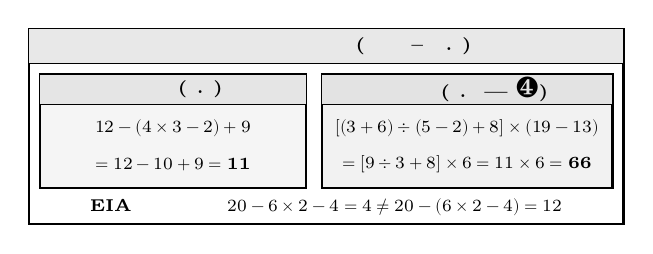
\begin{tikzpicture}[x=1cm, y=1cm, every node/.style={font=\fontsize{6.2pt}{8.2pt}\selectfont, text=black}]
  \draw[black, line width=0.9pt] (0,0) rectangle (7.55,2.48);
  \fill[gray!18] (0,2.04) rectangle (7.55,2.48);
  \draw[black, line width=0.6pt] (0,2.04) -- (7.55,2.04);
  \node at (3.775,2.26) {\textbf{ការគណនាកន្សោមមានវង់ក្រចក និងដង្កៀប (ឧទាហរណ៍ ៦--៧ ទំ.១០)}};

  % Left: Ex 6
  \draw[black, line width=0.8pt, fill=gray!8] (0.14,0.46) rectangle (3.52,1.90);
  \fill[gray!20] (0.14,1.52) rectangle (3.52,1.90);
  \draw[black, line width=0.5pt] (0.14,1.52) -- (3.52,1.52);
  \node at (1.83,1.71) {\textbf{ឧទាហរណ៍ ៦ (ទំ.១០)}};
  \node at (1.83,1.22) {$12 - (4\times 3 - 2) + 9$};
  \node at (1.83,0.76) {$= 12 - 10 + 9 = \mathbf{11}$};

  % Right: Ex 7
  \draw[black, line width=0.85pt, fill=gray!10] (3.72,0.46) rectangle (7.41,1.90);
  \fill[gray!22] (3.72,1.52) rectangle (7.41,1.90);
  \draw[black, line width=0.5pt] (3.72,1.52) -- (7.41,1.52);
  \node at (5.565,1.71) {\textbf{ឧទាហរណ៍ ៧ (ទំ.១០ — \cnum{4})}};
  \node at (5.565,1.22) {$[(3+6)\div(5-2)+8]\times(19-13)$};
  \node at (5.565,0.76) {$= [9\div 3 + 8]\times 6 = 11\times 6 = \mathbf{66}$};

  \node at (3.775,0.21) {\textbf{\en{EIA}៖} បើគ្មានវង់ក្រចក៖ $20-6\times 2-4 = 4 \ne 20-(6\times 2-4) = 12$};
\end{tikzpicture}}

% ៥. E5 Evaluate: សំណួរវិនិច្ឆ័យ A-D លើ 30 - 10 : 2 x 3
\newcommand{\figExitWNOneFive}{%
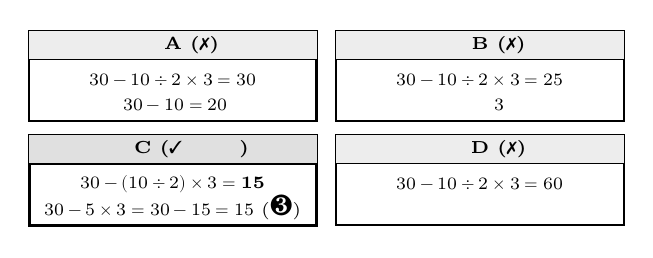
\begin{tikzpicture}[x=1cm, y=1cm, every node/.style={font=\fontsize{6.3pt}{8.2pt}\selectfont, text=black}]
  % Choice A
  \draw[black, line width=0.8pt] (0,1.32) rectangle (3.65,2.46);
  \fill[gray!14] (0,2.10) rectangle (3.65,2.46);
  \draw[black, line width=0.5pt] (0,2.10) -- (3.65,2.10);
  \node at (1.825,2.28) {\textbf{ជម្រើស \en{A} (\ding{55})}};
  \node at (1.825,1.84) {$30 - 10 \div 2 \times 3 = 30$};
  \node at (1.825,1.53) {ច្រឡំដក $30-10=20$ មុនចែក};

  % Choice B
  \draw[black, line width=0.8pt] (3.90,1.32) rectangle (7.55,2.46);
  \fill[gray!14] (3.90,2.10) rectangle (7.55,2.46);
  \draw[black, line width=0.5pt] (3.90,2.10) -- (7.55,2.10);
  \node at (5.725,2.28) {\textbf{ជម្រើស \en{B} (\ding{55})}};
  \node at (5.725,1.84) {$30 - 10 \div 2 \times 3 = 25$};
  \node at (5.725,1.53) {ភ្លេចគុណនឹងកត្តា $3$ ចុងក្រោយ};

  % Choice C (Correct)
  \draw[black, line width=1.05pt] (0,0) rectangle (3.65,1.14);
  \fill[gray!24] (0,0.78) rectangle (3.65,1.14);
  \draw[black, line width=0.6pt] (0,0.78) -- (3.65,0.78);
  \node at (1.825,0.96) {\textbf{ជម្រើស \en{C} (\ding{51} ត្រឹមត្រូវ)}};
  \node at (1.825,0.52) {$30 - (10\div 2)\times 3 = \mathbf{15}$};
  \node at (1.825,0.22) {$30 - 5\times 3 = 30 - 15 = 15$ (\cnum{3})};

  % Choice D
  \draw[black, line width=0.8pt] (3.90,0) rectangle (7.55,1.14);
  \fill[gray!14] (3.90,0.78) rectangle (7.55,1.14);
  \draw[black, line width=0.5pt] (3.90,0.78) -- (7.55,0.78);
  \node at (5.725,0.96) {\textbf{ជម្រើស \en{D} (\ding{55})}};
  \node at (5.725,0.52) {$30 - 10 \div 2 \times 3 = 60$};
  \node at (5.725,0.22) {ច្រឡំដកមុន និងគុណខុសលំដាប់};
\end{tikzpicture}}

\begin{document}
\fontsize{10pt}{15.2pt}\selectfont

% ============================================================================
% ក្បាលរដ្ឋបាល (Administrative Header — តាមគំរូ ls_plan.tex)
% ============================================================================
{\centering
  {\muol\fontsize{11pt}{16pt}\selectfont ព្រះរាជាណាចក្រកម្ពុជា\par}
  {\muol\fontsize{11pt}{16pt}\selectfont ជាតិ សាសនា ព្រះមហាក្សត្រ\par}
  \vspace{-3pt}{\khmflourish\par}
}

\vspace{1pt}
{\muol\fontsize{10pt}{15.5pt}\selectfont
មន្ទីរអប់រំ យុវជន និងកីឡា ខេត្តកំពង់ធំ\par
ការិយាល័យអប់រំ យុវជន និងកីឡា ស្រុកកំពង់ស្វាយ\par
អនុវិទ្យាល័យព្រះក្រសាំង\par}

\vspace{2pt}
{\centering{\muol\fontsize{11.5pt}{17pt}\selectfont កិច្ចតែងការបង្រៀន\par}}
\vspace{2pt}

% --- ព័ត៌មានទូទៅ ---
{\hspace*{2.8cm}\renewcommand{\arraystretch}{1.08}
\begin{tabular}{@{}l@{\hspace{0.35cm}}p{2.9cm}@{\hspace{0.15cm}}c@{\hspace{0.25cm}}l@{}}
  - & មុខវិជ្ជា & : & គណិតវិទ្យា ថ្នាក់ទី៧ (ពីជគណិត) \\
  - & ចំណងជើងមេរៀន & : & មេរៀនទី១៖ ចំនួនគត់ \\
  - & ចំណងជើងរង & : & ៦. លំដាប់នៃប្រមាណវិធីលើចំនួនគត់ (ទំ.៩--១០) \\
  - & រយៈពេល & : & ១ ម៉ោងសិក្សា (៥០ នាទី) \\
  - & បង្រៀនដោយ & : & ហុក ប៊ុនថែន \\
  - & កាលបរិច្ឆេទ & : & ថ្ងៃសៅរ៍ ទី៧ ខែវិច្ឆិកា ឆ្នាំ២០២៦ \\
\end{tabular}\par}

\vspace{2pt}

% --- I. វត្ថុបំណង ---
{\muol\fontsize{10pt}{15.5pt}\selectfont \enbf{I.} វត្ថុបំណង\par}
\vspace{1pt}
{\renewcommand{\arraystretch}{1.10}
\begin{tabular}{@{}p{0.55cm}@{}p{2.35cm}@{\hspace{0.15cm}}c@{\hspace{0.25cm}}p{14.95cm}@{}}
  \hfill\wcirc\hspace{0.2cm} & វិជ្ជាសម្បទា & : & សិស្សប្រាប់បានច្បាស់ពីវិធានលំដាប់នៃប្រមាណវិធីលើចំនួនគត់ ទាំងកន្សោមមានតែវិធីបូកនិងដក មានតែវិធីគុណនិងចែក មានប្រមាណវិធីទាំងបួន និងមានវង់ក្រចក $(\dots)$ ព្រមទាំងដង្កៀប $[\dots]$ បានត្រឹមត្រូវ ។ \\
  \hfill\wcirc\hspace{0.2cm} & បំណិនសម្បទា & : & សិស្សគណនាតម្លៃនៃកន្សោមលេខចម្រុះតាមជំហានអាទិភាពដោយប្រើសញ្ញាផ្ដុំពីក្រោម ($\underbrace{\quad}$) លើសន្លឹកកិច្ចការបានត្រឹមត្រូវតាមគំរូសៀវភៅគោល (ឧទាហរណ៍ ១--៧ ទំ.៩--១០) ។ \\
  \hfill\wcirc\hspace{0.2cm} & ចរិយាសម្បទា & : & សិស្សមានវិន័យនិងភាពម៉ត់ចត់ក្នុងការពិនិត្យអាទិភាពប្រមាណវិធីមុនគណនា មិនធ្វើតាមទម្លាប់ស្មាន និងចេះផ្ទៀងផ្ទាត់ជំហានគណនាគ្នាទៅវិញទៅមកជាក្រុម ។ \\
\end{tabular}\par}

\vspace{2pt}

% --- II. សម្ភារៈឧបទេស ---
{\muol\fontsize{10pt}{15.5pt}\selectfont \enbf{II.} សម្ភារៈឧបទេស\par}
\vspace{1pt}
\hspace*{0.55cm}$\bullet$\ សៀវភៅសិក្សាគោលថ្នាក់ទី៧ (ទំ.៩--១០ និងទំ.១៤) ក្ដារខៀន ដីស/ហ្វឺត បន្ទាត់ត្រង់ និង\textbf{សន្លឹកកិច្ចការសិស្សបំពេញចន្លោះ ស-ខ្មៅ} (កូដ \en{WN15} ទំព័រ ១--២ សម្រាប់សិស្ស និងទំព័រ ៣ ប្លង់ក្ដារខៀន/ចម្លើយគ្រូ — គ្មានប្រើ \en{LCD})\par

\vspace{2pt}

% --- III. វិធីសាស្រ្តបង្រៀន ---
{\muol\fontsize{10pt}{15.5pt}\selectfont \enbf{III.} វិធីសាស្រ្តបង្រៀន\par}
\vspace{1pt}
{\renewcommand{\arraystretch}{1.08}
\begin{tabular}{@{}p{0.55cm}@{}p{2.35cm}@{\hspace{0.15cm}}c@{\hspace{0.25cm}}p{14.95cm}@{}}
  \hfill$\bullet$\hspace{0.2cm} & គោលវិធី & : & សិស្សមជ្ឈមណ្ឌល (សន្លឹកកិច្ចការបំពេញចន្លោះជាគោល + ការពិភាក្សាជាក្រុមតូច ៣ នាក់) \\
  \hfill$\bullet$\hspace{0.2cm} & យុទ្ធវិធីបង្រៀន & : & គំរូស្ថាបនានិយម \en{5Es} រួមបញ្ចូល \textbf{ការវិភាគដំណោះស្រាយខុសទល់នឹងត្រូវ (\en{Erroneous Worked-Example Critique})} និង \textbf{គំនូសផ្ដុំតាមជំហាន (\en{Underbrace Step-Tracing})} \\
\end{tabular}\par}

\vspace{2pt}

% --- IV. ដំណើរការបង្រៀន ---
{\muol\fontsize{10pt}{15.5pt}\selectfont \enbf{IV.} ដំណើរការបង្រៀន\par}

{\renewcommand{\arraystretch}{1.15}
\begin{longtable}{|L{5.50cm}|L{7.90cm}|L{4.80cm}|}
\hline
\multicolumn{1}{|c|}{\cellcolor{headgray}\muol សកម្មភាពគ្រូ} &
\multicolumn{1}{c|}{\cellcolor{headgray}\muol ខ្លឹមសារមេរៀន} &
\multicolumn{1}{c|}{\cellcolor{headgray}\muol សកម្មភាពសិស្ស} \\
\hline
\endfirsthead

\hline
\multicolumn{1}{|c|}{\cellcolor{headgray}\muol សកម្មភាពគ្រូ} &
\multicolumn{1}{c|}{\cellcolor{headgray}\muol ខ្លឹមសារមេរៀន} &
\multicolumn{1}{c|}{\cellcolor{headgray}\muol សកម្មភាពសិស្ស} \\
\hline
\endhead

% ==================== ជំហានទី១ (2min) ====================
\stepheader{ជំហានទី១ \enbf{(}រដ្ឋបាលថ្នាក់\enbf{)}}
$\bullet$ ពិនិត្យវត្តមាន អនាម័យ និងសណ្ដាប់ធ្នាប់ថ្នាក់រៀន \par
$\bullet$ រៀបចំក្រុមតូច ៣ នាក់តាមតុ និងចែក\textbf{សន្លឹកកិច្ចការសិស្ស (\en{WN15} ទំព័រ ១–២)}
&
$\bullet$ រដ្ឋបាលថ្នាក់ អនាម័យ និងវិន័យសិក្សា \par
$\bullet$ ចែកសន្លឹកកិច្ចការម្នាក់ ១ សន្លឹក សម្រាប់បំពេញតាមដំណាក់កាល \en{E1--E5}
&
$\circ$ ប្រធានថ្នាក់រាយការណ៍វត្តមានសិស្ស \par
$\circ$ ទទួលសន្លឹកកិច្ចការ សរសេរឈ្មោះ និងអង្គុយតាមក្រុម ៣ នាក់ \\
\hline

% ==================== ជំហានទី២ (9min: កំណែ <=3m + រំលឹក 3m + E1 3m) ====================
\stepheader{ជំហានទី២ \enbf{(}កិច្ចការផ្ទះ \enbf{+} ទំនាក់ទំនងមេរៀនថ្មី\enbf{)}}
\ditem \textbf{កំណែកិច្ចការផ្ទះ ($\le\text{\enbf{3\,min}}$)} \par
$\bullet$ ហៅសិស្សឡើងកែលំហាត់ទំ.១៤ លេខ ២ ក និងលំហាត់គណនារហ័សលើក្ដារខៀនផ្នែកឆ្វេង
&
{\centering\redsub{កំណែកិច្ចការផ្ទះមេរៀនមុន (ទំ.១៤ លេខ ២ ក និងគណនារហ័ស)}\par}
$\bullet$ \textbf{ទំ.១៤ លេខ ២ ក៖} $40\times 5 + 50\times 6 - 7\times 60 = 200 + 300 - 420 = \mathbf{80}$ \par
$\bullet$ \textbf{គណនារហ័ស៖} ក. $\mathbf{1\,900}$ \quad ខ. $\mathbf{3\,700}$ \quad គ. $\mathbf{594}$
&
$\circ$ ផ្ទៀងចម្លើយ ($80; 1\,900; 3\,700; 594$) និងកែចូលសៀវភៅ \\[3pt]

\ditem \textbf{រំលឹកមេរៀនទាក់ទង (\enbf{3min})} \par
$\bullet$ លើកស្ថានភាពពិត៖ «បើប្អូនមានប្រាក់ $19$ ម៉ឺនរៀល ចាយអស់ $3$ ម៉ឺនរៀល រួចឪពុកឱ្យថែម $7$ ម៉ឺនរៀល តើនៅសល់ប្រាក់ប៉ុន្មាន?»
&
{\centering\redsub{រំលឹកន័យនៃការដកនិងបូកបន្តបន្ទាប់ក្នុងជីវភាពពិត}\par}
$\bullet$ ជំហានទី១ (ចាយអស់ $3$ ម៉ឺន)៖ $19 - 3 = 16$ ម៉ឺនរៀល \par
$\bullet$ ជំហានទី២ (បានថែម $7$ ម៉ឺន)៖ $16 + 7 = \mathbf{23}$ ម៉ឺនរៀល
&
$\circ$ ឆ្លើយ៖ «នៅសល់ $16$ ម៉ឺន បូកថែម $7$ ម៉ឺន ស្មើ $23$ ម៉ឺនរៀល!» \\[3pt]

$\bullet$ សួរបន្ត៖ «ចុះកន្សោម $40\times 5 + 50\times 6$ ក្នុងកិច្ចការផ្ទះមិញ ហេតុអ្វីយើងគុណមុនបូក?»
&
$\bullet$ ព្រោះ $40\times 5$ និង $50\times 6$ ជាបណ្ដុំផលគុណដែលត្រូវរកតម្លៃមុនយកមកបូកបញ្ចូលគ្នា
&
$\circ$ រំលឹកថាផលគុណត្រូវគណនាមុនផលបូក \\[3pt]

\fiveE{E1 - Engage (3min)} \timenote{(កុំទាន់ផ្ដល់ចម្លើយ)} \par
\ditem \textbf{បេសកកម្មវិភាគដំណោះស្រាយខុសទល់នឹងត្រូវ (សន្លឹកកិច្ចការ \en{E1})} \par
$\bullet$ ឱ្យសិស្សពិនិត្យប្រអប់ \en{E1} លើកន្សោម $19 - 3 + 7$ (ឧទាហរណ៍ ១ ទំ.៩) រវាង\textbf{សិស្ស ក} និង\textbf{សិស្ស ខ}
&
\redsub{បេសកកម្ម \en{E1}៖ គណនា $19 - 3 + 7$ (ឧទាហរណ៍ ១ ទំ.៩)} \par
$\bullet$ \textbf{សិស្ស ក (បូកមុន)៖} $19 - (3 + 7) = 19 - 10 = 9$ \par
$\bullet$ \textbf{សិស្ស ខ (ពីឆ្វេងទៅស្ដាំ)៖} $(19 - 3) + 7 = 16 + 7 = 23$ ។ តើអ្នកណាត្រូវ?
&
$\circ$ ពិភាក្សាជាគូ និងគូស \ding{51} ក្នុងប្រអប់ \en{E1} លើសន្លឹកកិច្ចការ \\[3pt]

&
\cfig{\figEngageWNOneFive}
& \\
\hline

% ==================== ជំហានទី៣ (17min: E2 11m + E3 6m) ====================
\stepheader{ជំហានទី៣ \enbf{(}ខ្លឹមសារមេរៀនថ្មី\enbf{)}}
\fiveE{E2 - Explore (11min)} \par
$\bullet$ សរសេរចំណងជើងរង \textbf{៦. លំដាប់នៃប្រមាណវិធីលើចំនួនគត់} លើក្ដារខៀន \par
\ditem \textbf{សកម្មភាព ១៖ កន្សោមមានតែ $+, -$ ឬមានតែ $\times, \div$ (ទំ.៩, \enbf{5min}, \en{E2-A})} \par
$\bullet$ ឱ្យសិស្សគូសសញ្ញាផ្ដុំពីក្រោម ($\underbrace{\quad}$) និងគណនាឧទាហរណ៍ ២, ៣, ៤ លើ \en{E2-A}
&
៦. លំដាប់នៃប្រមាណវិធីលើចំនួនគត់ \par
$\bullet$ \textbf{ឧទាហរណ៍ ២ (ទំ.៩)៖} $\underbrace{12 - 2}_{10} + 10 - 14 = \underbrace{10 + 10}_{20} - 14 = \mathbf{6}$ \par
$\bullet$ \textbf{ឧទាហរណ៍ ៣ និង ៤ (ទំ.៩)៖} $\underbrace{6 \times 12}_{72} \div 4 = \mathbf{18}$; \quad $\underbrace{125 \div 5}_{25} \times 15 = \mathbf{375}$
&
$\circ$ គូសផ្ដុំពីឆ្វេងទៅស្ដាំឃើញ $6$, $18$ និង $375$ លើ \en{E2-A} \\[3pt]

$\bullet$ សួរឆ្លុះបញ្ចាំងលើឧទាហរណ៍ ៤៖ «បើច្រឡំគុណ $5 \times 15 = 75$ មុន តើ $125 \div 75$ ចែកដាច់ឬទេ?»
&
$\bullet$ កត់សម្គាល់៖ $125 \div 75$ មិនចែកដាច់ជាចំនួនគត់ទេ! បញ្ជាក់ថា $\div$ និង $\times$ ត្រូវធ្វើពីឆ្វេងទៅស្ដាំ
&
$\circ$ ឃើញច្បាស់ថាមិនអាចធ្វើគុណមុនចែកតាមទំនើងចិត្តទេ \\[3pt]

\ditem \textbf{សកម្មភាព ២៖ កន្សោមមានប្រមាណវិធីទាំងបួន (ឧទាហរណ៍ ៥ ទំ.៩, \enbf{6min}, \en{E2-B})} \par
$\bullet$ ឱ្យសិស្សគូសផ្ដុំបណ្ដុំគុណនិងចែកជាមុនក្នុងកន្សោម $52 - 4\times 12 + 18\div 6\times 3$ លើ \en{E2-B}
&
$\bullet$ \textbf{ឧទាហរណ៍ ៥ (ទំ.៩)៖} គណនា $52 - 4 \times 12 + 18 \div 6 \times 3$ \par
\hspace*{0.2cm}$= 52 - \underbrace{4 \times 12}_{48} + \underbrace{18 \div 6}_{3} \times 3 = \underbrace{52 - 48}_{4} + \underbrace{3 \times 3}_{9} = 4 + 9 = \mathbf{13}$
&
$\circ$ គូសផ្ដុំ $4\times 12=48$ និង $18\div 6\times 3=9$ រួចគណនាឃើញ $13$ \\[3pt]

&
\cfig{\figStepTraceWNOneFive}
& \\[3pt]

% --- E3 Explain (6min) ---
\fiveE{E3 - Explain (6min)} \par
$\bullet$ ដឹកនាំសិស្សសង្ខេបវិធានជាទូទៅទាំង ៤ កម្រិត (ទំ.៩--១០) លើសន្លឹកកិច្ចការ \en{E3}
&
$\bullet$ \textbf{វិធានជាទូទៅនៃលំដាប់ប្រមាណវិធី (ទំ.៩--១០)៖} \par
\hspace*{0.15cm}១) មានតែវិធីបូកនិងដក ឬមានតែវិធីគុណនិងចែក $\to$ គណនា\graybox{ពីឆ្វេងទៅស្ដាំ} \par
\hspace*{0.15cm}២) មានប្រមាណវិធីទាំងបួន $\to$ ធ្វើ \graybox{$\times$ ឬ $\div$} មុន \graybox{$+$ និង $-$} ពីឆ្វេងទៅស្ដាំ
&
$\circ$ បំពេញពាក្យគន្លឹះក្នុងប្រអប់វិធានលើ \en{E3} \\[3pt]

$\bullet$ បង្ហាញវិធានកន្សោមមានវង់ក្រចក $(\dots)$ និងដង្កៀប $[\dots]$ (ទំ.១០)
&
\hspace*{0.15cm}៣) មានវង់ក្រចក និងដង្កៀប $\to$ ធ្វើក្នុង \graybox{$(\dots)$} មុន រួចធ្វើក្នុង \graybox{$[\dots]$}
&
$\circ$ បំពេញលំដាប់ $(\dots) \to [\dots]$ លើ \en{E3} \\[3pt]

$\bullet$ ភ្ជាប់\textbf{ធនាគារហេតុផល \cnum{1}--\cnum{2}} សម្រាប់ប្រមាណវិធីកម្រិតស្មើគ្នា
&
\cnum{1} \textbf{កម្រិតស្មើគ្នា $(+, -)$៖} គណនាតាមលំដាប់ពីឆ្វេងទៅស្ដាំ \par
\cnum{2} \textbf{កម្រិតស្មើគ្នា $(\times, \div)$៖} គណនាតាមលំដាប់ពីឆ្វេងទៅស្ដាំ
&
$\circ$ ផ្ទៀងលេខកូដ \cnum{1}--\cnum{2} លើសន្លឹកកិច្ចការ \\[3pt]

$\bullet$ ភ្ជាប់\textbf{ធនាគារហេតុផល \cnum{3}--\cnum{4}} សម្រាប់កន្សោមចម្រុះ និងវង់ក្រចក/ដង្កៀប
&
\cnum{3} \textbf{ប្រមាណវិធីទាំងបួន៖} ធ្វើគុណ ឬចែកមុនបូកនិងដក ពីឆ្វេងទៅស្ដាំ \par
\cnum{4} \textbf{វង់ក្រចក និងដង្កៀប៖} ធ្វើក្នុង $(\dots)$ មុន រួចក្នុង $[\dots]$ ទើបចេញក្រៅ
&
$\circ$ ផ្ទៀងលេខកូដ \cnum{3}--\cnum{4} លើសន្លឹកកិច្ចការ \\[3pt]

&
\cfig{\figHierarchyWNOneFive}
& \\
\hline

% ==================== ជំហានទី៤ (20min: E4 10m + E5 10m) ====================
\stepheader{ជំហានទី៤ \enbf{(}ពង្រីកចំណេះដឹង\enbf{)}}
\fiveE{E4 - Elaborate (10min)} \par
\ditem \textbf{ឧទាហរណ៍គំរូ ៦ និង ៧៖ វង់ក្រចក និងដង្កៀប (សៀវភៅគោល ទំ.១០)} \par
$\bullet$ ឱ្យសិស្សគណនាឧទាហរណ៍ ៦ ($12 - (4\times 3 - 2) + 9$) តាមជំហានលើ \en{E4}
&
{\muol ឧទាហរណ៍ ៦} \textbf{(ទំ.១០ — កន្សោមមានវង់ក្រចក)៖} \par
$\bullet$ $12 - (\underbrace{4 \times 3}_{12} - 2) + 9 = 12 - (\underbrace{12 - 2}_{10}) + 9 = \underbrace{12 - 10}_{2} + 9 = \graybox{$11$}$ (\cnum{4}, \cnum{1})
&
$\circ$ គណនាគុណក្នុងវង់ក្រចកមុន ($12-2=10$) រួចឃើញ $11$ \\[3pt]

$\bullet$ ឱ្យសិស្សគណនាឧទាហរណ៍ ៧ ($[(3+6)\div(5-2)+8]\times(19-13)$) លើ \en{E4}
&
{\muol ឧទាហរណ៍ ៧} \textbf{(ទំ.១០ — កន្សោមមានវង់ក្រចក និងដង្កៀប)៖} \par
$\bullet$ $[(\underbrace{3+6}_{9}) \div (\underbrace{5-2}_{3}) + 8] \times (\underbrace{19-13}_{6}) = [\underbrace{9 \div 3}_{3} + 8] \times 6 = 11 \times 6 = \graybox{$66$}$ (\cnum{4})
&
$\circ$ គណនាវង់ក្រចកទាំងបី រួចដង្កៀប $[3+8]=11$ គុណនឹង $6$ ឃើញ $66$ \\[3pt]

&
\cfig{\figBracketsWNOneFive}
& \\[3pt]

$\bullet$ សួរសំណួរឆ្លុះបញ្ចាំង \textbf{\en{EIA Looking-Back} (1min)} ប្រៀបធៀបវត្តមានវង់ក្រចក
&
\textbf{\en{EIA Looking-Back}៖} «ប្រៀបធៀប $20 - (6\times 2 - 4)$ និង $20 - 6\times 2 - 4$ តើវង់ក្រចកប្ដូរលទ្ធផលដូចម្ដេច?» ($\to 20 - 8 = \mathbf{12}$ ខុសពី $20 - 12 - 4 = \mathbf{4}$!)
&
$\circ$ បកស្រាយតួនាទីវង់ក្រចកក្នុងការប្ដូរលំដាប់អាទិភាព \\[3pt]

% --- E5 Evaluate (10min) ---
\fiveE{E5 - Evaluate (10min)} \par
\ditem \textbf{ប្រតិបត្តិជាក្រុមតូច ៣ នាក់ (4min, សន្លឹកកិច្ចការ \en{E5})} \par
$\bullet$ ឱ្យក្រុមសិស្សគណនាកន្សោមអនុវត្តន៍ ក និង ខ លើសន្លឹកកិច្ចការ \en{E5}
&
{\muol លំហាត់ប្រតិបត្តិអនុវត្តន៍} \textbf{(ត្រៀមភ្ជាប់លំហាត់ទំ.១៤ លេខ ២)៖} \par
$\bullet$ \textbf{ក.} $48 \div 6 \times 4 - (15 - 3) \div 3 = 8 \times 4 - 12 \div 3 = 32 - 4 = \graybox{$28$}$ \par
$\bullet$ \textbf{ខ.} $[(14 + 6) \div 5 + 6] \times (15 - 8) = [20 \div 5 + 6] \times 7 = 10 \times 7 = \graybox{$70$}$
&
$\circ$ សហការគ្នាគណនាតាមជំហានឃើញ $28$ និង $70$ \\[3pt]

$\bullet$ ឱ្យក្រុមសិស្សផ្ទៀងផ្ទាត់និង\textbf{បិទបេសកកម្ម \en{E1} (2min)}
&
$\bullet$ \textbf{បិទបេសកកម្ម \en{E1}៖} \textbf{សិស្ស ខ} ត្រឹមត្រូវ! $19 - 3 + 7 = 16 + 7 = \mathbf{23}$ (\cnum{1}) ព្រោះវិធីដកនិងវិធីបូកត្រូវធ្វើពីឆ្វេងទៅស្ដាំ ។
&
$\circ$ បិទបេសកកម្ម \en{E1} ឃើញសិស្ស ខ ត្រឹមត្រូវ ($23$) \\[3pt]

\ditem \textbf{សំណួរវិនិច្ឆ័យ \en{A--D} និងសំបុត្រចេញ (4min)} \par
$\bullet$ សរសេរកន្សោម $30 - 10 \div 2 \times 3$ និងជម្រើស \en{A--D} លើក្ដារខៀន
&
{\centering\textbf{សំណួរវិនិច្ឆ័យ \en{A--D}៖ តើតម្លៃនៃកន្សោម $30 - 10 \div 2 \times 3$ ស្មើនឹងប៉ុន្មាន?}\par}
&
$\circ$ គណនា $10\div 2 = 5$, $5\times 3 = 15$, រួច $30 - 15 = 15$ \\[3pt]

$\bullet$ ឱ្យសិស្សគូសរង្វង់ជម្រើសត្រូវលើសន្លឹកកិច្ចការ រួចលើកម្រាមដៃ ១--៤ ព្រមគ្នា
&
$\bullet$ វិភាគកំហុសក្នុងជម្រើស \en{A} ($30$), \en{B} ($25$), \en{D} ($60$) តាមលេខកូដហេតុផល \cnum{2} និង \cnum{3}
&
$\circ$ គូសរង្វង់លើសន្លឹកកិច្ចការ និងលើកម្រាមដៃ ៣ (\textbf{ជម្រើស \en{C}}) \\[3pt]

&
\cfig{\figExitWNOneFive}
& \\[3pt]

$\bullet$ បញ្ជាក់ចម្លើយត្រូវ (\textbf{ជម្រើស \en{C}}) និងឱ្យបំពេញ\textbf{សំបុត្រចេញ ៦០ វិនាទី}
&
$\bullet$ \textbf{សំបុត្រចេញ៖} $24 \div (8 - 2) + 5 \times 3 = 24 \div 6 + 15 = 4 + 15 = \mathbf{19}$ (\cnum{3}, \cnum{4}) ។
&
$\circ$ បំពេញសំបុត្រចេញឃើញ $19$ មុនបញ្ចប់ម៉ោង \\
\hline

% ==================== ជំហានទី៥ (<=2min) ====================
\stepheader{ជំហានទី៥ \enbf{(}កិច្ចការផ្ទះ \enbf{+} បណ្ដាំផ្ញើ\enbf{)}}
\timenote{ចំណាយពេលឱ្យតិចបំផុតកុំឱ្យលើស 2min} \par
$\bullet$ ណែនាំប្រអប់\textbf{កិច្ចការផ្ទះ}លើសន្លឹកកិច្ចការទំព័រ ២ (សៀវភៅគោល ទំ.១៤ លេខ ២ ខ, គ, ឃ, ង)
&
{\centering{\muol កិច្ចការផ្ទះ} \textbf{(សៀវភៅគោល ទំ.១៤ លេខ ២ ខ, គ, ឃ, ង)}\par} \par
$\bullet$ \textbf{ខ.} $(57 + 43 - 7 \times 5) \times 20 + 4 \times 90$ \quad \textbf{គ.} $56 \div 8 + (47 - 17) \div 5 - 13$ \par
$\bullet$ \textbf{ឃ.} $[4 \times 15 + 72 \div 8 - (47 - 23) \div 6] \times 2$ \par
$\bullet$ \textbf{ង.} $75 - 38 \div 2 + 75 \div 5 \times 7 + 81 \div 3 \div 9 \times 7 - 15 + 6 \times 7$
&
$\circ$ គូសចំណាំលំហាត់ទំ.១៤ លេខ ២ ខ, គ, ឃ, ង \\[3pt]

$\bullet$ ផ្ដាំផ្ញើឱ្យធ្វើកិច្ចការផ្ទះតាមជំហាន និងអានមុនចំណុច ៧ (ទំ.១០–១១)
&
$\bullet$ \textbf{បណ្ដាំផ្ញើ៖} គូសសញ្ញាផ្ដុំពីក្រោមពេលធ្វើកិច្ចការផ្ទះ និងអានមុន \textbf{៧. ការបង្គត់ចំនួនគត់ និងការប៉ាន់ស្មាន} (ទំ.១០–១១) ។
&
$\circ$ កត់ត្រាបណ្ដាំផ្ញើ ទុកសន្លឹកកិច្ចការក្នុងសៀវភៅ និងជម្រាបលាគ្រូ \\
\hline
\end{longtable}}

\vspace{6pt}
% --- ហត្ថលេខា (កាលបរិច្ឆេទត្រូវគ្នា ១០០% នឹងខាងលើ) ---
{\centering
\hspace*{5.2cm}\begin{minipage}{11.5cm}
  \centering
  ថ្ងៃសៅរ៍ ១២រោច ខែអស្សុជ ឆ្នាំមមី អដ្ឋស័ក ពុទ្ធសករាជ ២៥៧០\par
  កំពង់ស្វាយ, ថ្ងៃទី៧ ខែវិច្ឆិកា ឆ្នាំ២០២៦\par
  \vspace{2pt}
  {\muol គ្រូបង្រៀន\par}
  \vspace{32pt}
  \hfill{\muol ហុក ប៊ុនថែន}\hspace*{1.4cm}
\end{minipage}\par}

\end{document}
